% reducesymm/blog/flotsam2modes.tex
% $Author$ $Date$

% Predrag 2014-07-14

\section{Draft write up flotsam}
\label{chap:flotsam2modes}

\noindent
{\bf [2012-04-26 Predrag]}
{\color{red}
Draft of \refref{BuBoCvSi14} flotsam; most recent clippings at the top.

How to use this section? When you remove cogent text from the article
proper - clip  it and paste it into here, for possible reuse later.
}
\bigskip\bigskip

Previous titles:

{\em A tutorial on the periodic orbit theory of the systems with continuous
symmetries}

{\em Symmetry reduction of the 1:2 spatial resonance with broken reflection
symmetry via the \mslices}

{\em Cartography of a 4-dimensional flow with a continuous symmetry:
- How to slice it}

{\em Rotational symmetry reduction of a model of mode-interactions via the
\mslices}

\begin{description}

\item[2013-07-25  Predrag] This is \BBedit{an example of Burak's edit},
and here is an internal footnote\BB{An internal footnote by Burak.}. They
are useful when you change something n the middle of a text, rather then
just append the newest blog post. Please remove the color from my
\PCedit{edits} as you read them and approve them, and I'll do the same
for yours.

% \item[2013-08-13  Predrag to Burak] Please define \eqv, \reqv, \po,
% and \rpo\ here, in form suitable for pasting into the putative
% \twoMode\ slicing paper.

\item[2014-05-27 Evangelos]
\refRef{gatermannHab} is
somewhat dated and probably nowdays people can find bases for $d>12$, but
I have not kept up with the literature. Do you have any newer
reference?

\item[2013-08-14  Predrag]
Your definition of a \reqv\ is correct for one-parameter $\Group$, but we
will have to rethink it for $N$\dmn\ Lie group $\Group$. In that case the
time trajectory is a 1\dmn\ curve, generically tracing out the $N$\dmn\
group orbit quasiperiodically. Probably a
\HREF{http://www.streamsound.dk/book1/chaos/chaos.html\#205/z} {better
definition} (click on magenta hyperlinks!) would be that
$\vel({\ssp_{\ssp}}) \in \pS_{EQ}$, and than show that this is then true
true anywhere on the group orbit. Perhaps using
\HREF{http://www.streamsound.dk/book1/chaos/chaos.html\#204/z} {Lie
derivatives}...

\item[2013-08-13 Burak]
\noindent{\bf Invariant solutions:}                     \toCB
A point $\ssp_{EQ}$ is an \eqv\ if the velocity function evaluated at this
point is 0, namely, $\dot{\ssp}|_{\ssp=\ssp_{EQ}} = \vel({\ssp_{EQ}}) = 0$.
Orbit of
a point $\ssp$ of a $\Group$-equivariant flow is called a \reqv\ if for any
time evolved point on the orbit $\ssp(\tau) = f^{\tau}(\ssp_{REQ})$ there
exists a parameter $\phi$ such that $\ssp(\tau) = \Group(\phi) \ssp$, in other
words, a time orbit is a \reqv\ if it coincides with the group orbit.
 A
point $\ssp$ is on a \po\ if its trajectory passes through itself after some
certain time \period{}, namely $\ssp = f^{\period{}}(\ssp)$. Finally, a point $\ssp$ of a
$\Group$-equivariant flow is said to be on a \rpo\ if there exists a
point $\ssp(\period{}) = f^\period{}(\ssp)$ on the orbit of $\ssp$, such that it satisfies $\ssp(\period{}) =
\LieEl(\phi) \ssp$ for a certain $\phi$.

\textbf{[2013-09-30  Predrag]}
Experimenting with how to compare parameter sets, starting with the set
\refeq{eq:PKparamsfinal}
\bea
\mu_1&=&-2.8023, \mu_2=1, a_1=-1, a_2=-2.6636
    \continue
b_1  &=& 0, b_2=0, c_1=-4.1122, c_2=1.8854, e_2=1
\,.
\label{eq:PKparamsfinal1}
\eea

\begin{tabular}{l|l|l|}
  & \refeq{eq:PKparamsfinal} & . \\
  \hline
  % after \\: \hline or \cline{col1-col2} \cline{col3-col4} ...
  $\mu_1$ & -2.8023 & . \\
  $\mu_2$ & 1       & . \\
  $e_1$   & 0       & 0 \\
  $e_2$   & 1       & . \\
  $a_1$   & -1      & . \\
  $a_2$   & -2.6636 & . \\
  $b_1$   & 0       & . \\
  $b_2$   & 0       & . \\
  $c_1$   & -4.1122 & . \\
  $c_2$   & 1.8854  & . \\
  $\#_{eqv}$ & . & . \\
  \hline
\end{tabular}


\end{description}

% former siminos/cgang/flotsam.tex    master file: main.tex
% $Author$ $Date$

% \section{Flotsam}
% \label{s:flotsam}


ES2014-05-27: Dropped this from intro: the reconstruction equations
developed in \refref{rowley_reconstruction_2000} and formulated them using a `rescaled
time' variable. Replaced with: Later on, Rowley \etal~\rf{rowley_reduction_2003}
generalized the method in order to handle self-similar solutions. -- Consider returning
to intro if we talk about rescaled time in more detail.



The basic equivariants include
\beq
  \{{z}_1\,,\overline{z}_1 {z}_2 \}
            \,,\qquad
  \{{z}_2 \,, z_1 \overline{z}_2\}
\,.
%\label{Dang86(1.3)PK}
\eeq
We have equations \refeq{eq:DangSO2} for $\{{z}_1\,,\overline{z}_1\,,
{z}_2\,,\overline{z}_2 \}$ but perhaps need equations for the
equivariants \refeq{Dang86(1.3)PK} - have not thought this through.
[ChaosBook.org says:]

%[2013-10-07 Burak]
Differential operators acting on functions defined on a periodic domain
usually diagonalized by representing the solution as a Fourier expansion.

%[2013-10-30 Burak] cut from 2modes.tex :
\PC{notation for the translation group?}
As at least 3 dimensions are required for a continuous time flow to
exhibit chaos, in this case the \statesp\ of a $\Group$-equivariant flow
has to be at least 4\dmn. Under linear actions of $\SOn{2}$ the \statesp\
decomposes into 2\dmn\ irreducible subspaces (Fourier components) labeled
by integers $m = 0,1,2,\cdots$, which thus form the natural basis in which
to study $\SOn{2}$-equivariant flows. Nonlinear flows, such as the
1 spatial dimension \KS\ PDE for a `flame front velocity' field
$u=u(x,t)$ on a periodic domain $u(x,t) = u(x+L,t)$, given by
\beq
  u_t = F(u) = -{\textstyle\frac{1}{2}}(u^2)_x-u_{xx}-u_{xxxx}
    \,,\qquad   x \in [-L/2,L/2]
    \,,
\ee{BBks1}
can be
expressed in terms of complex Fourier coefficients $a_k(t)$,
\beq
  u(x,t)=\sum_{k=-\infty}^{+\infty} a_k (t) e^{ i q_k x}
\,,\qquad
  q_k = 2\pi k/L
\,,
\ee{BBeq:ksexp1}
as
\beq
\dot{a}_k= \pVeloc_k(a)
     = ( q_k^2 - q_k^4 )\, a_k
    - i \frac{q_k}{2} \sum_{m=-\infty}^{+\infty} a_m a_{k-m}
\,.
\ee{2m:expan}
($t \geq 0$ is the time, $x$ is the spatial coordinate, subscripts $x$
and $t$ denote partial derivatives with respect to $x$ and $t$).
Nonlinear terms mix an infinity of
Fourier components. In practice, they are represented by truncations to
a finite number of Fourier modes; the most radical truncation that
still might capture some qualitative features of a chaotic flow is to keep
only a pair of Fourier modes.


%[2013-11-06 Burak] cut from 2modes.tex :
\bea
  w  &=& - \frac{2\,u}{c_1}\,A_1 = - \frac{2\,v}{c_2}\,A_2
\continue
        &\to&\quad 2\,A_1+ A_2 = - \frac{ w}{2\,u\,v}\left(c_2\,u+2\,c_1\,v\right)
\continue
  q  &=& \frac{1}{-2e_1+e_2}
     \left(- {w^2}/{2\,u\,v} + \,2u\right)\left(c_2\,u+2\,c_1\,v\right)
%\label{PKinvEqs4}
\\
  w  &=& -\frac{1}{-2e_1+e_2} (2\,A_1+ A_2)\,q
     \,,\quad\to\quad
  q = \frac{2(-2e_1+\,e_2)\,u\,v}{c_2\,u+2\,c_1\,v}
  \,,
\nnu
\eea

%[2013-11-06 Burak] cut from 2modes.tex :
and thus we obtain \textbf{our main result}, two (bivariate)  polynomials
in two variables $\{u,v\}$ with constant coefficients
\bea
f(u,v) &=&
  c_2\,u\,(\mu_1+a_1\,u+b_1\,v)
     -
  c_1\,v\,(\mu_2+a_2\,u+b_2\,v) = 0 %Double checked DB 04-30-2012
\,,\qquad  deg(f) = 2
\continue
g(u,v) &=&
 \left(w^2 - 4\,u^2 v\right)\left(c_2\,u+2\,c_1\,v\right)^2 %Double checked DB 04-30-2012
 +\,4\,(-2e_1+e_2)^2\,u^2\,v^2 = 0
\,,\qquad  deg(g) = 6
\,,
%\label{PKinvEqs5}
\eea

%[2013-11-08 Burak] cut from 2modes.tex :

where $w$ is defined by the first equation in
\refeq{PKinvEqs4}.

Lots of coefficients, but we can
absorb some into rescaled quantities
$\tilde{u} = c_2\,u$,
$\tilde{v} = c_1\,v$,
$\tilde{a_1} = a_1/c_2$,
$\tilde{b_1} = b_1/c_1$,
$\tilde{a_2} = a_2/c_2$,
$\tilde{b_2} = b_2/c_1$,
and by using $A_1$ expression for $w$ factored out the pair of $u=0$
roots:

so we are down to 8 coefficients. Note that $e_2 \in \reals_{+}$, and if
we agree that  $\mu_1 > -\mu_2 > 0$ we can rescale the first equation so
that in new time units $\tilde{\mu}_1 =1$, $\tilde{\mu}_2 = \mu_2/\mu_1
\in \reals_{-}$, so there are 7 coefficients in all. I see no further
rescaling simplification.

As we already know $[0,0,0,0]$ and $[0,v,0,0]$ roots, one should divide
them out, and that is what we have done. Finding
roots of bivariate polynomials is not easy.

{\bf[2014-05-06 Burak]} I'll try to rewrite the abstract from the beginning,
here is its current version:
\newline
Dangelmayr\rf{Dang86} and Porter~\&\ Knobloch\rf{PoKno05} have
introduced a family of 2-Fourier mode \SOn{2}-equivariant ODEs  in order to
study bifurcations of solutions of dynamical systems in presence of
symmetries. A 4\dmn\ system of this kind is perhaps the simplest
example of a system with a continuous symmetry that can exhibit chaos, so
we use it to illustrate the role symmetries play in chaotic dynamics. We
show that a continuous symmetry induces drifts in the full
{\statesp} dynamics, drifts which obscure the chaotic dynamics. Change of
equations of motions to a {\comovframe} frame
does not eliminate these drifts: that is only attained by a
\emph{symmetry reduction} - reformulation of dynamics in a 3-dimensional
symmetry-reduced {\statesp}, where every group orbit (set of all points
reached by actions of the group of all symmetries of the equations of
motion) is replaced by a point. {\twoMode} system is a
particularly nice illustration of how this works, as in 3 dimensions we
are able to visualize everything.

We compare three symmetry reduction methods: polar coordinates, invariant
polynomial bases, and the `{\mslices}'. An invariant polynomial
basis is convenient for determination of all {\reqva} of such
system. Our conclusion, however, is that the most insight is offered by
the {\mslices}. While in general a number of local slices are
needed to cover a strange attractor\rf{atlas12}, for the {\twomode}
system there we define a unique slice hyperplane that captures
\emph{all} symmetry-reduced dynamics. \BBedit{I think this is misleading
since we have shown that single slice treatment works fine for \KS }

A Poincar\'e return map within the
slice hyperplane enables us to reduce the dynamics further, essentially
to a unimodal map, and determine, in principle, all {\rpo s} of the system.
We can visualize each step of this process without
having to project solutions onto a submanifold since the slice hyperplane
for this system is three dimensional.

{\bf[2014-05-06 Burak]} Previously was in introduction, later commented
out:
\newline
Over the last decade, new insights into the dynamics of  [blah blah]

Our goals here are two-fold:
    \PC{{\bf[2013-10-07]} Burak's and Daniels outline of Das Artikel is
in \reffig{fig:131007outline}.
}
(i)  Illustrate \mslices\ in the lowest\dmn\ setting possible.
(ii) [blah blah].

As a motivation, consider the chaotic dynamics exhibited by the
small-cell \KS\ system studied in \refref{lanCvit07}. Examination of
typical long-time simulations shows that the spatio-temporal chaos arises
from visits to two kinds of unstable patterns, a `central wobble' region
$S_C$, and a symmetric pair of right/left `drifts' $\{S_L,S_R\}$. In
\statesp\ projections orbits stay in one neighborhood for a while, then
hop to another neighborhood, as illustrated in \reffig{f:antlong}. The
strange attractor that they explore is curved and folded in such a way
that a single local linear chart cannot cover the whole attractor,
several charts are needed, as illustrated by \reffig{fig:2ModeAtlas}\,(d).

The \statesp s of \KS\ and fluid-dynamical flows are high\dmn\ and
difficult to visualize, so here we shall illustrate the key ideas by a
much simpler example, the $\SOn{2}$-equivariant  \twomode\ system.

%%%%%%%%%%%%%%%%%%%%%%%%%%%%%%%%%%%%%%%%%%%%%%%%%%%%%%%%%%%%
\begin{figure} %[tbp] %[h]
    \centering
 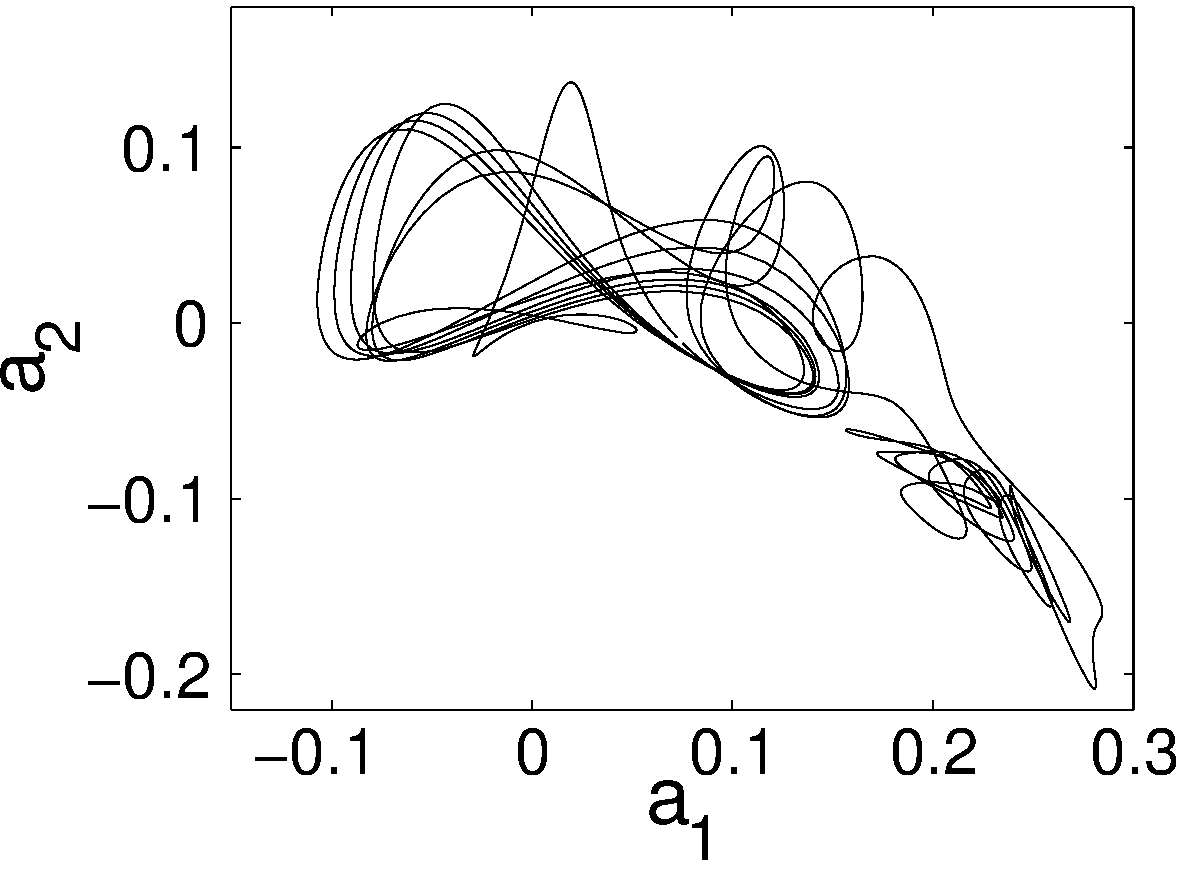
\includegraphics[width=0.40\textwidth]{kslong12}
\caption[]{
A long \KS\ \po\ of period $\period{}=355.34$ that connects
neighborhoods called `$S_C$' and `$S_R$',
(c) $[a_1,a_2]$  projection on the first two spatial Fourier modes
(from \refref{lanCvit07}).
      }
\label{f:antlong}
\end{figure}
%%%%%%%%%%%%%%%%%%%%%%%%%%%%%%%%%%%%%%%%%%%%%%%%%%%%%%%%%%%%%%

 [blah blah]


{\bf[2014-05-06 Burak]} Previous outline items:

SO2-equivariant equations:
\bea
\dot{x}_1 &=& (\mu_1 - r_1^2 + c_1 x_2)x_1 + c_1 y_1 y_2
\continue
\dot{y}_1 &=& (\mu_1 - r_1^2 - c_1 x_2)y_1 + c_1 x_1 y_2
\continue
\dot{x}_2 &=& (1 + a_2 r_1^2)x_2 + (x_1^2 - y_1^2) + y_2
\continue
\dot{y}_2 &=& (1 + a_2 r_1^2)y_2 + 2 x_1 y_1 - x_2
\continue
		  && \mbox{where } r_1^2 = x_1^2 + y_1^2\, , \quad r_2^2 = x_2^2 + y_2^2
\,.
\label{2mode4Dset1}
\eea


%%%%%%%%%%%%%%%%%%%%%%%%%%%%%%%%%%%%%%%%%%%%%%%%%%%%%%%%%%%%%%%%%%%%%%%%%%%%%%%%%%%%%%%%%%%%%%%%%
\subsection{To do}
\label{s:ToDo}

\begin{itemize}
  \item[10.11] Visualizations of the 4-dimensional {\twomode} system
  \item[10.1?] draw a group orbit for the {\twomode} model
  \item[10.22] {\twoMode} system in polar coordinates (maybe skip)
  \item[10.23] The \reqva\ of the {\twomode} system
  \item[10.24] Plotting the \reqva\ of
           the {\twomode} system in invariant coordinates
  \item[10.25] Plotting the \reqva\ of
           the {\twomode} system in Cartesian coordinates
           \refeq{2mode4D}
  \item[10.2?] construct a 2-chart atlas
           \reffig{fig:2ModeAtlas} for a {\twomode} system
  \item
        compute analytically the \stabmat\ \Mvar\ in polar coordinates
  \item
        Study eigenvalues, keep playing with parameters. We would like
        -preferably- no \reqv\ to be attracting limit cycle, and several of
        the \reqva\ to be complex-pair unstable, leading to chaos, to be
        visualized and sliced in Cartesian coordinates.
  \item
        If you find a nice chaotic attractors, others can join in
        constructing an atlas for it. We just need one and only one
        example with non-trivial \chartBord s and at least 2 charts.
\end{itemize}

 [blah blah]

\begin{itemize}
  \item $\REQV{}{1} = (r_1,r_2,\psi)=(0.0516508, 1.26311,?)$ and
        $\REQV{}{2} = (0.467095,0.2146,?)$
  \item their plots in the Cartesian coordinates
  \item $\dot{\theta}$ to see how slow/fast are they. $\dot{\theta}$
        might be related to 4th eigenvalue, when you go back
        to Cartesian coordinates
  \item stability eigenvalues, eigenvectors of the \eqv\ $\EQV{0}$ at
        origin, at your parameter values - if it is stable, everything
        just might fall into it and die.
  \item plots of small perturbations of the above \eqv\ and \reqva\ in
        the Cartesian coordinates to see whether the dynamics looks
        chaotic
  \item $\REQV{}{1}$: 2 large positive eigenvalues looks scary - probably
        nothing re-visits this \reqv. A mildly unstable complex pair
        would have been sweeter. You get complex eigenvalue by Hopf-bifurcating off a
        stable orbit, typically.
  \item $\REQV{}{1}$: Does either unstable eigenvalue become a complex
        eigenvalue pair in Cartesian coordinates?
  \item $\REQV{}{2}$: contracting eigenvalues have very small imaginary
        part, so the presumably just rocket toward the \reqv, not much
        spiraling there. At least the unstable eigenvalue seems slow
        compared to all other eigenvalues.
  \item $\REQV{}{1}$: Does the unstable eigenvalue become a complex
        eigenvalue pair in Cartesian coordinates?
\end{itemize}

 [blah blah]



%%%%%%%%%%%%%%%%%%%%%%%%%%%%%%%%%%%%%%%%%%%%%%%%
 2011-09-09, 2012-03-30 Predrag: add BeThMovFr to
            continuous.tex overheads, and ChaosBook
 replace A27movFrame*.* everywhere
\begin{figure}
  	\begin{center}
(a)
(b)
(c)
(d)
    \end{center}
  \caption{
  \twoMode, $d=4 \to 3$~dimensional $\{x_1,x_2,z\}$ projections:
  (a)
  The strange attractor.
  (b)
 (c)
 In contrast
 to the 1\dmn\ \poincBord s of \reffig{fig:2modeSects}, here ...
 (d)
  }
\label{fig:2ModeAtlas}
\end{figure}
%%%%%%%%%%%%%%%%%%%%%%%%%%%%%%%%%%%%%%%%%%%%%%%%%

 [blah blah]

 [blah blah]

\section{Chart}
\label{s:slice}

 [blah blah]

One can write the equations for the flow in the \reducedsp\
$\dot{\sspRed} = \velRed(\sspRed)$ (for details see, for example,
\refref{DasBuch}) as
\bea
\velRed(\sspRed) &=& \vel(\sspRed)
     \,-\, \dot{\gSpace}(\sspRed) \, \groupTan(\sspRed)
\label{2modesEqMotMFrame}\\
\dot{\gSpace}(\sspRed) &=& \braket{\vel(\sspRed)}{\sliceTan{}}
                       /\braket{\groupTan(\sspRed)}{\sliceTan{}}
\,
\label{2modesreconstrEq}
\eea
which confines the motion to the \slice\ hyperplane. Thus, the dynamical
system $\{\pS,\map^t\}$ with continuous symmetry \Group\ is replaced by
the {\reducedsp} dynamics $\{\pSRed,\mapRed^t\}$: The velocity in the
full \statesp\ $\vel$ is the sum of $\velRed$, the velocity component in
the \slice\ hyperplane, and $\dot{\gSpace}\,\groupTan$, the velocity
component along the group tangent space. The integral of the {\em
reconstruction equation} for $\dot{\gSpace}$ keeps track of the group
shift in the full \statesp.


 [blah blah]

{\bf[2014-05-07 Burak]} Taken out from \refsect{s-slice}:
\newline

\refFig{fig:BBgorbitsandslice} shows a 3D projection of the 4D \statesp\ corresponding
to an $m=2$ truncation of \refeq{FourierSeries}, for which \refeq{mmodeLieEl} and \refeq{mmodeLg}
are $4 \times 4$ matrices. The \slicePlane\ defined by \refeq{firstmodetemp}, three
different group orbits and the group tangents evaluated at their intersections with the \slicePlane\
are visualized in \reffig{fig:BBgorbitsandslice}. One can see as the magnitude of the second mode (the vertical axis)
relative to the first mode increases, the group tangent gets closer to being
parallel to the \slicePlane , however, it still has a non zero perpendicular component. The vertical
axis ($x_2$) in \reffig{fig:BBgorbitsandslice} lies on the \sliceBord\ of the
\slicePlane .

{\bf[2014-06-25 Burak]} Taken out from \refsect{s-numerics}:
\newline

We start with the first set of parameters\ES{2014-05-15}{Will you also show the second set? If not,
you might as well drop it and stick with a single set. If there is nothing interesting to
be seen, then maybe keep it simple.}, \refeq{eq:pars}.

% If this ever comes back use brackets consistent with \verbatim{\invpt} for \invpt{u,v,w,q} points
%  			  &=& \left[0,- \infty,0,0\right]
% 			  \continue
% 			  &=& \left[-2.8,0,0,0\right]
% 			  \continue
% 			  &=& \left[-5.52172,0.12361,-3.87834,0.183536\right]
% 			  \continue
% 			  &=& \left[-0.991847 \mp 0.14571 \ii,
% 				   \ceq
% 				   -0.0640782 \pm 0.00260791 \ii,
% 				   \ceq
% 				   0.468295 \pm 0.0306953 \ii,
% 				   \ceq
% 				   -0.067488 \pm 0.687486 \ii\right]
% \eea


Starting close to the {\reqv} \REQV{1},
we integrate the $\SOn{2}$-equivariant
equations \refeq{2mode4D} for 500 time units and plot two projections of the 4D
\statesp\ in \reffig{fig:2modes-conf-reqv}\,(a) and \reffig{fig:2modes-conf}\,(b). In order to compare the symmetry
reduction techniques, we plotted the corresponding flow in the invariant polynomial
basis on \reffig{fig:2modes-conf}(c) and the symmetry reduced flow using \mslices\
on \reffig{2modes-ssp}. While \reffig{fig:2modes-invpol}
 is generated by simply
integrating \refeq{PKinvEqs1}, we obtained \reffig{2modes-ssp1} by integrating
\refeq{eq:so2reduced} within the \slicePlane\ of the \template,
\beq
	\slicep = (1,0,0,0)
\label{eq:firstmodetemplate}
\eeq
with the same initial condition $x_0$ (note that it satisfies \refeq{SliceCond}
for \refeq{eq:firstmodetemplate} and \refeq{LGTwoMode}) and

The Poincar\'e section plane in \reffig{fig:BBpsecthd} includes the origin \PC{??}
and is
perpendicular to
\beq
	\hat{n}_{0,GS} = (0, -0.54030, 0.84147)
	\label{eq:nhat0GS-1}
\eeq

\begin{figure}%[H]
  \begin{center}
  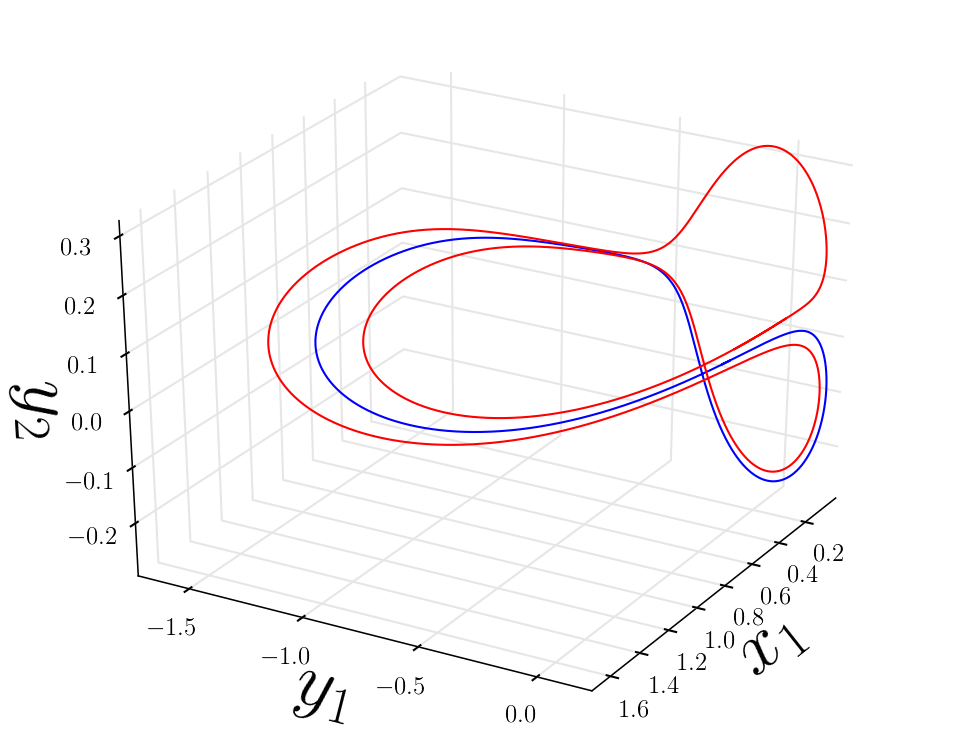
\includegraphics[width=0.45\textwidth]{BBrpo}
  \end{center}
  \caption{
	\Rpo s \cycle{1} and \cycle{01} embedded in the strange attractor
    of \reffig{fig:psectandretmap}\,(a).
    }
  \label{fig:BBrpo1-01}
\end{figure}

\rpo s and their binary itineraries, the two shortest cycles
\cycle{1} and \cycle{01} are plotted in
\reffig{fig:BBrpo1-01}.

{\bf[2014-06-25 Burak]} Taken out from \label{s-mframes}:

An immediate generalization of the transformation \refeq{e-1stmodeTransform},
is to fix the phase of a higher Fourier mode rather than that of the first one; this, however, requires
some extra care as we shall explain for the second Fourier mode.
Consider the phase-fixing transformation,
\beq
	\sspRedC_n = e^{-\ii n \frac{\phi_2}{2}} \sspC_n \, ,
	\label{e-2ndmodeTransform}
\eeq
which fixes the phase of the second mode to $0$. Note, however, that since
$\phi_2 \in (0, 2 \pi]$ it can have discontinuities of $2 \pi$. This means
that when the first Fourier mode is transformed, it will have a phase discontinuity
of $\pi$. This discontinuity can be fixed by another
transformation:
\bea
	\tilde{\sspC}_1 &=& e^{-\ii 2 \hat{\phi}_1} |\sspRedC_1 | \, , \continue
	\tilde{\sspC}_{n \neq 1} &=& \sspRedC_n \, ,
	\label{e-PhaseDoubling}
\eea
where we simply doubled the phase $\hat{\phi}_1$ of the symmetry-reduced
first mode $\sspRedC_1$, obtained by \refeq{e-2ndmodeTransform} and left
the rest of the modes unchanged. Combination of \refeq{e-2ndmodeTransform}
and \refeq{e-PhaseDoubling} is a valid symmetry reduction scheme since every
group orbit is represented by a single point, furthermore, it is also continuous
and revertible hence one can make further computations, such as constructing
Poincar\'{e} sections, using this form. For the 2-mode case at hand, representation
\refeq{e-PhaseDoubling} does not have any particular advantage against
\refeq{e-1stmodeTransform}, however, for higher dimensional flows, second
(or higher) Fourier mode subspaces can have dynamical importance as shown in
\refref{SCD07}. In order to capture those regions of the \statesp\ this
representation would be a useful alternative.

{\bf[2014-07-06 Burak]} Previous abstract:

In nonlinear flows drifts along symmetry directions often obscure the
physical, `shape changing' dynamics. Symmetry reduction eliminates such
drifts through a coordinate transformation that parametrizes motions along
symmetry directions by `phase' coordinates and maps symmetry-related \statesp\ points
to single points in a symmetry-reduced \statesp.

Here, we illustrate and compare
three different symmetry reduction methods: polar coordinates, invariant
polynomial bases, and the `{method of slices}' by applying them to a
simple dynamical system
%
\DBedit{- a chaotic flow based on the normal form of the 1:2 spatial resonance
with broken reflection symmetry}
%
\DB{2014-05-15}{Is there anything called a normal form flow? I don't
think so but I could be wrong. I know `normal forms' and I know `flows'
but not `normal form flows'. Refering to 1:2 resonance might also peak a
certain crowd's interest, even though we don't really do anything in a
regime that they would care about. Talking about broken symmetry is
sexier than talking about SO(2).}
\ES{2014-05-20}{Talking about broken symmetry in the title of a paper on
symmetry reduction could also be misleading. Important is not which
symmetry is broken, but which symmetry we reduce, right? 1:2 resonance
sounds cryptic to me, I would prefer to say mode interaction. Have a look
at edited title. }
%
 - that can be thought of as a truncation of a spatially extended PDE. We find that the {method
of slices} offers the most insight.  Because the flow is four dimensional,
the slice hyperplane for this system is three dimensional, which allows
the visualization of each step of the symmetry-reduction process without having to
project the dynamics onto lower-dimensional submanifolds. A Poincar\'e return
map within the slice hyperplane enables further reduction of the dynamics to what is effectively a unimodal map, allowing (in principle) the determination of all {\rpo s} of the system.

{\bf[2014-07-07 Burak]} Previous introduction:

Recent experimental observations of travelling waves in pipe flows have confirmed predictions based on dynamical systems theory that coherent structures play an important role in shaping the \statesp\ of turbulent flows\rf{science04}. Identifying such solutions can lead to a better
understanding of the transition to turbulence in fluid flows and may, in the long-term,
allow the computation of dynamical averages using periodic orbits. In order to
find coherent solutions such as \reqva\ and \rpo s it is essential, as we shall demonstrate,
to use continuous symmetry reduction.

One well-studied technique for symmetry reduction, which works well for low-dimensional dynamical systems such
as Lorenz and R\"{o}ssler flows, is to recast the dynamical equations in terms of invariant polynomials\rf{GL-Gil07b}.
However, establishing an invariant polynomial basis becomes impractical
for systems with more than 12 dimensions\rf{gatermannHab}\ES{2014-05-27}{\refref{gatermannHab}
is somewhat dated and probably nowdays people can find bases for $d>12$,
but I have not kept up with the literature. Do you have any
newer reference?}.
The \mslices%
\rf{rowley_reconstruction_2000,BeTh04,SiCvi10,FrCv11,atlas12,ACHKW11,BudCvi14},
which we study in detail here, offers a symmetry reduction
scheme applicable to high-dimensional flows like the \NS\ equations.

While the \mslices\ goes back to Cartan\rf{CartanMF}, to the
best to our knowledge, Rowley and Marsden\rf{rowley_reconstruction_2000}
were first to apply it to spatially extended nonlinear flows.
They demonstrated their method by applying it to the one-dimensional \KS\ equation
in a periodic domain and used it to study its dynamics in the neighborhood of
a \reqv\ by using the \reqv\ itself as the \slice\ `\template'. Later on,
Rowley \etal~\rf{rowley_reduction_2003} generalized the method in order
to handle self-similar solutions. Beyn and Th\"{u}mmler\rf{BeTh04} applied
the \mslices\ to `freeze' spiral waves in reaction-diffusion systems.

These early studies applied the \mslices\ to a single solution at a time, but
studying the nonlinear dynamics of extended systems requires symmetry reduction
of global objects, such as strange attractors or invariant manifolds.
In this spirit, Siminos and Cvitanovi\'{c}\rf{SiCvi10} used the \mslices\ to
quotient the \SOn{2} symmetry of chaotic dynamics in \cLf\ and showed that the
slice-dependent singularity of the reconstruction equation
causes the reduced flow to make discontinuous jumps. This singularity was studied
in detail by Froehlich and Cvitanovi\'{c}\rf{FrCv11}.

Two strategies have been proposed in order to handle this problem: either to
try to identify a template such that slice singularities are not visited
by dynamics\rf{SiCvi10} or to use multiple `charts' of connected
slices\rf{rowley_reconstruction_2000,FrCv11}.
The latter approach was applied to \cLf\ by Cvitanovi\'{c} \etal~\rf{atlas12} and
to pipe flow by Willis, Cvitanovi\'{c}, and Avila\rf{ACHKW11}.
\ESedit{However, neither approach is straightforward to apply, particularly in
high-dimensional dynamical systems.
More recently, Budanur \etal\rf{BudCvi14} considered Fourier space discretizations of
PDEs, in which translational symmetry naturally appears as the rotation group
\SOn{2}. They showed that a simple choice of \slice, associated to the first Fourier mode,
results in a \slice\ singularity that generic dynamics is extremely improbable to visit.}
\ES{2014-06-03}{rephrased this to make easier to follow for the casual reader:
followed a geometrical approach
and showed that for \SOn{2} a specific choice of a \slice\
\template\ can be used to move the \slice\ singularity to the border of the
symmetry-reduced submanifold.
}
Close-passages to the
singularity were regularized by means of a time rescaling. Here, we follow this approach
and apply \ESedit{this so-called ``first Fourier mode slice''} method
to a 2-mode ODE normal form, which may be
the simplest system with \SOn{2} equivariant dynamics
that exhibits chaos.

{\bf[2014-07-14 Burak]} Taken out from \refsect{s:eqva}:
\newline

In order to find \reqva\ of the \twomode\ system, one has to solve two bivariate
polynomials \refeq{PKinvEqs5a} which, in general, is not a trivial task. However,
as we shall see in the examples of the next section, for particular choices
of parameters, equations\refeq{PKinvEqs5a} symplify significantly allowing
us to determine all \reqva\ of the \twomode\ system.

{\bf[2014-07-14 Burak]} Taken out from \refsect{s:numerics}:
\newline

To illustrate the \mslices\ on the \twomode\ system we choose a simple
set of parameters for which we observe interesting dynamics. These
parameters are listed in \refeq{eq:pars}. With this set of parameters,
we can write \twomode\ ODEs \refeq{eq:DangSO2} in terms of three parameters
$\{ \mu_1, c_2, a_2 \}$:
\bea
\label{eq:DangSO2set1}
  \sspC_1 &=& \mu_1 \,z_1 - z_1|z_1|^2 +c_1\,\overline{z}_1\,z_2
  \continue
  \sspC_1 &=& (1-\ii)\,{z_2}+a_2\,z_2|z_1|^2+\,z_1^2
\,,
\eea
Note that by setting $b_2 = 0$, we send the \reqv\ at
$\cartpt{0,-\mu_2/b_2,0,0}$ to infinity. Moreover, \refeq{PKinvEqs5a}
yields
$\tilde{v} = (\mu_1 + \tilde{a}_1 \tilde{u})/(\mu_2 + \tilde{a}_2
\tilde{u} - \tilde{u} \tilde{b}_1)$. Substitution into \refeq{PKinvEqs5b}
allows one to solve for a single variable. By solving \refeq{PKinvEqs5}
with the parameter set \refeq{eq:pars}, we get two real roots, with
non-negative $u$ and $v$:
%the \eqva\ of the system in the invariant polynomial basis \refeq{Dang86(1.2)PK} as
\[
	\invpol_{\EQV{}} = (0,0,0,0)^T %\qquad \mbox{(double)}
\]
which is a double root and corresponds to an equilibrium of \refeq{eq:DangSO2}, and
\[
			 \invpol_{\REQV{}{}} = (0.193569,0.154131,-0.149539,-0.027178)^T\,,
\]
which is a {\reqv}. In real representation, a
representative point on  \REQV{}{} may be chosen as
\[
  \left(x_1, y_1, x_2, y_2\right) = \left(0.439966, 0, -0.386267, 0.070204\right)
\]


{\bf[2014-07-15 Burak]} Taken out from \refsect{s:flow}:
\newline

\PC{2014-07-14
Why $\pm L/2$ in \reffig{fig:2modes-conf} and
\reffig{fig:2modes-conf-reqv} and not $\pm \pi$?
}
\ES{2014-05-15}{I have replaced the second-mode slice, double-angled
figure in \reffig{2modes-conf-reqv}\,(b) with one resulting by integrating on the
$(0,0,1,0)$ slice, for consistency with panel (c). I hope Burak will
replace it with a publication quality figure of the same representation.
The trick of angle doubling will be introduced in its own section. }

{\bf[2014-07-15 Burak]} Took out from the lead paragraph:
\PCedit{ % Jul 14 2014
Burak, have a look at Chaos Journal articles. This section is required,
and most of your abstract goes into it, the abstract itself should be concise:
``Today, it is possible to  [blah blah]''.
    }

{\bf[2014-07-15 Burak]} Abstract before divison:

Periodic orbit theory provides estimates for dynamical
averages, such as dissipation rates or diffusion constants, of nonlinear
flows by means of {\cycForm s} which relate the spectra of observables
to the spectra of unstable periodic orbits. These formulas are valid
under the assumption that the periodic orbits have a single marginal
direction along the time evolution, and hyperbolic in all other
directions. Dynamical systems with continuous symmetries, however, have
relative periodic orbits which are invariant $(N+1)$ dimensional tori, where $N$
is the number of continuous symmetries. These systems arise in the study
of turbulent flows, such as Navier-Stokes in a pipe or plane Couette
flow, where one often imposes periodic boundary conditions along the
stream direction and truncates the corresponding infinite Fourier series
to a finite but large number (from tens to thousands) Fourier modes. In
this paper we study a `\twomode' model of this type,
the smallest possible truncation with a 4\dmn\ \statesp,
which has the same continuous symmetry structure as the $1D$ PDE
while just high-dimensional enough to allow for chaotic dynamics.
The
crucial step in analysis of such systems is symmetry reduction, here a
coordinate transformation that separates physical, `shape changing'
dynamics from the drifts along the symmetry direction. We start by
reviewing continuous symmetries and symmetry reduction methods with a
focus on the `\mslices ', which, to the best of our knowledge, is the
only symmetry reduction method that can be applied to the infinite
dimensional problems. We then define our \twomode\ \SOn{2}-equivariant
model, compare different symmetry-reduction schemes, and determine its
\reqva\ using invariant polynomials. We show that a Poincar\'e section
within the `\slice' can be used to further reduce this flow to what is
for all practical purposes a
unimodal map; and hence we can find all \rpo s and their binary symbolic
dynamics up to any desired period.
We finally compute dynamical averages using \rpo s, and discuss
convergence of the spectral determinants.

{\bf[2014-08-04 Burak]} Took out from \refsect{s-mframes}:

\DBedit{We immediately see that the reconstruction phase in \refeq{eq:so2reduced}
is, for this particular \slice, the phase of the first mode without the
symmetry reduction.}
\DB{2014-05-15}{I don't immediately see what we are saying here. How does
this relate to \refeq{eq:so2reduced}? I think this needs better
explanation.}
\ES{2014-05-15}{It's not straightforward to see this, also for me, unless
I think of the postprocessing approach. So I have added \refeq{eq:phi1}
above. Please check and discuss in the blog if needed.}
%
\DB{2014-05-15}{This phrase has no meaning.}
\BB{2014-05-15}{Is it better know?}
%
As the magnitude of the first mode,
$\sqrt{\hat{x}_1^2 + \hat{y}_1^2}$, relative to that of the second mode becomes smaller,
its group tangent has a larger component parallel to the \slicePlane. The \sliceBord\ condition
\refeq{ChartBordCond} is satisfied when the group tangent becomes parallel to the \slicePlane.
%
\DB{2014-05-15}{Don't love my wording of ``parallel to the \slicePlane'' since some people might interpret the
\slicePlane\ as being defined by a vector normal to its surface and hence a perpendicular to the
group tangent at the \sliceBord. However, I think that ``component that lies within the slice'' is
sort of vague and not well defined mathematically. What do you guys think?}

{\bf[2014-08-05 Burak]} Took out from \refsect{s:twoMode}:

Our goal is to illustrate and compare continuous symmetry reduction methods
applicable to high-dimensional systems exhibiting chaos.


{\bf[2014-10-30 Burak]} From introduction:
This mode mixing phenomenon
\DB{9/16/2014}{Is the mixing really the source of \rpo s and \reqva ? It seems
to me that this statement isn't necessarily true right?}
\BB{9/17/2014}{You are right, mode mixing is just a consequence of the
nonlinearity, not necessarily the cause of the \rpo s and \reqva. You can
change as you see fit}
\BB{10/30/2014}{Changed myself.}

Section {\em Post-processing approach} refers to the ``method of moving
frames'' (postprocessing approach) and as such belongs here. It has to be
generalized a bit (I will do it if you agree with the change). Second
mode \slice\ can be used also for integration on the \slice\ and can be
introduced earlier.

{\bf[2014-05-15 Evangelos]} Why do you count complex solutions as equilibria?

{\bf[2014-11-07 Burak]} Took out the partial derivative from this
sentence (Mohammad's suggestion: `Everybody knows the chain rule.'):

\( %beq
 \dot{ u}_i= \sum_j ({\partial u_i}/{\partial \ssp_j}) \, \dot{\ssp}_j
 \,,
\) %ee{HilbChainRl}


More explicit form, does not fit in a column:
\[
	 \LieEl (\theta)= \\
					  \begin{pmatrix}
					  \cos \theta & \sin \theta & 0               & 0              & \cdots & 0              & 0               \\
					 -\sin \theta & \cos \theta & 0               & 0              & \cdots & 0              & 0               \\
					  0             & 0 		   & \cos 2 \theta & \sin 2 \theta & \cdots & 0              & 0               \\
					  0             & 0            &-\sin 2 \theta & \cos 2 \theta & \cdots & 0              & 0               \\
					  \vdots       & \vdots      & \vdots         & \vdots        & \ddots & \vdots         & \vdots         \\
					  0             & 0 		   & 0               & 0              & \cdots & \cos m \theta & \sin m \theta  \\
					  0             & 0            & 0	             & 0              & \cdots &-\sin m \theta & \cos m \theta
					  \end{pmatrix}
\]


{\bf[2014-11-08 Predrag]} clipped some commented text from the manuscript
and to here:

\noindent
author{ Keith M. Carroll} \\%no response by 2013-08-28
author{ Bryce Robbins} \\%no response by 2012-07-26, readded 2013-08-28
author{ Evangelos Siminos}  \\ % not in groove with Burak
%Max-Planck Institute for the Physics of Complex Systems,
%N\"{o}thnitzer Str. 38, D-01187 Dresden, Germany}
author{ Lei Zhang} %no response by 2012-07-26, removed

{\bf[2014-09-16 Daniel]}
Should stability matrices and Jacobians be bolded like \Lg?

{\bf[2014-09-16 Burak]}
\Lg is bolded because in general it is $\Lg = (\Lg_1,
\Lg_2, ..., \Lg_N)$. Chaosbook convention is to use small letters for the
vectors in the \statesp , capital letters for the matrices that act on
the \statesp\ vectors (stability matrix, Jacobian etc), and bold capital
letters for set of matrices like \Lg . Current notation here is not
perfect. In general we have $N$ group parameters that determines the
group element as $g(\gSpace) = e^{\theta \cdot \Lg}$. I think easiest way
to get rid off this ambiguity is to say that we are formulating
everything for a single parameter group and than remove `\\bf' from the
macro for \Lg .

{\bf[2014-11-09 Predrag]}
 Daniel is right, ChaosBook.org choice of fonts is inconsistent.
Now I've revamped all matrices in blackboard font, but not the vectors
that really does not look good.

{\bf[2014-11-11 Daniel]}
There is some notational nastiness in the averages section,
since there are $\ssp'$ s
floating around. We have previously used $\ssp'$ for the template and
used primes in general mark template related things.\\
{\bf[2014-11-11 Predrag]} Grin and bear it.

{\bf[2014-11-11 Daniel]}
What is $T$ here... at this point in the paper $T$ has been used to
represent both period of cycles and Lie group generator. Okay... reading
further it's clearly a period, but we may want to fix this notational
ambiguity.\\
{\bf[2014-11-11 Predrag]} We are lucky that Chinese did not invent modern
mathematics. Otherwise we would have a unique ideogram for every concept.

{\bf[2014-11-11 Daniel]}
We say ``only the combination $(2e_1-e_2)$ matters in the symmetry reduced
dynamics, so for simplicity we set $e_1=0$''
and then never really do it in any of the analysis except in numerics.
Should we get rid of $e_1$ everywhere or keep it?\\
{\bf[2014-11-11 Predrag]} might revisit this in the next revision, no time for it now...

%\DBedit{DB: Not sure where this factor of 2 comes from in $w =
%-\frac{2}{e_2} (2\,A_1+ A_2)\,q $. From the last equation in
%\refeq{PKinvEqs3}, I get $w = -\frac{1}{e_2} (2\,A_1+ A_2)\,q$.
%Therefore, I get I get  $q = \frac{2 e_2\,u\,v}{c_2\,u+2\,c_1\,v}$}
%2012-04-29 Predrag: thanks!

% \DBedit{DB: I get $g(u,v) = \left(w^2 - 4\,u^2
% v\right)\left(c_2\,u+2\,c_1\,v\right)^2 +\,4\,e_2^2\,u^2\,v^2 = 0$}
%2012-04-29 Predrag: thanks!
%2012-04-29 Predrag: should have I used the syzygy \refeq{eq:syzPK},
%$w^2 - 4\,u^2v = -q^2$ DB: If you plug the syzygy in you trivially get zero....


{\bf[2014-11-11 Daniel]}
What does $\simeq$ mean in this context? Aren't they actually the same?
\\
{\bf[2014-11-11 Predrag]} They are isomorphic, but defining reps are different -
one is 1d complex, the other 2d real
